\documentclass[
	article,			% article académique
	11pt,				% taille de la police
	oneside,			% impression imprimante
	a4paper,			% taille du paper
	chapter=TITLE,
	french,			% langue
	sumario=tradicional
	]{base_nt}

\usepackage{comment}

\usepackage{titlesec}
\usepackage{titletoc}

\usepackage{pgfgantt}
\usepackage{xcolor}

\definecolor{myforestgreen}{RGB}{40, 167, 69}
\definecolor{myred}{RGB}{220, 53, 69}

% Redéfinit le style des \part pour supprimer les pages générées
\titleclass{\part}{top} % Utilise le style de section "top" pour les parties
% Modifie l'espacement avant le titre de la partie
\titlespacing*{\part}{0pt}{0pt}{0pt}

\titleformat{\part}[display]{\Huge}{}{-2cm}{}

% commande simple pour afficher les commandes Latex sous forme de texte
\newcommand{\comando}[1]{\textbf{$\backslash$#1}}

\titulo{Procédure d'installation/désinstallation}

\tituloestrangeiro{Projet par des étudiants de l'EPITA}

\autor{
Félix, Yanis, Hamza, Antoine et Keany Vy \thanks{Ce rapport a été élaboré dans le cadre d'un projet réalisé à l'EPITA - (École Pour l'Informatique et les Techniques Avancées) \url{epita.fr}} 
\\[0.5cm]
\href{mailto:keany-vy.khun@epita.fr}{keany-vy.khun@epita.fr}, \href{mailto:antoine.mulot@epita.fr}{antoine.mulot@epita.fr}
\\[0.5cm]
\href{mailto:felix.despretz@epita.fr}{felix.despretz@epita.fr}, \href{ mailto:yanis.jerjini@epita.fr}{yanis.jerjini@epita.fr}, \href{mailto:hamza.khamchane@epita.fr}{hamza.khamchane@epita.fr}
\\[0.3cm]
20 juin, 2024 }


\evento{EPITA Projet S2 - Promo 2028 - Studio NeedTime()} % Bandeau au dessus de toutes les pages
\local{France}
\data{Version 1.0.1 - prod}

\begin{document}

\selectlanguage{french}

\frenchspacing 

% ----------------------------------------------------------
% ELEMENTOS PRÉ-TEXTUAIS
% ----------------------------------------------------------

%---
%
% Se desejar escrever o artigo em duas colunas, descomente a linha abaixo
% e a linha com o texto ``FIM DE ARTIGO EM DUAS COLUNAS''.
% \twocolumn[    		% INICIO DE ARTIGO EM DUAS COLUNAS
%
%---
\maketitle

% ----------------------------------------------------------
% ELEMENTOS TEXTUAIS
% ----------------------------------------------------------
\textual

\newpage

\customtableofcontents

% ----------------------------------------------------------
% Introduction
% ----------------------------------------------------------
%\begin{comment}
\newpage

\part{Comment installer le jeu ?}
\section{Installation Windows x86}

Pour télécharger le launcher vous pouvez vous rendre directement sur notre site web.

\vspace{0cm}
\begin{figure}[ht]
	\caption{Site web}
	\centering
	\includegraphics[width=1\linewidth]{launcher_dl.png}
	\legend{Téléchargement : \url{https://needtime.pages.dev/download}}
	
\end{figure}

\newpage

Une fois le launcher téléchargé, vous devrez le lancer puis suivre les étapes suivantes.

\vspace{0cm}
\begin{figure}[ht]
	\caption{Gestionnaire de fichiers}
	\centering
	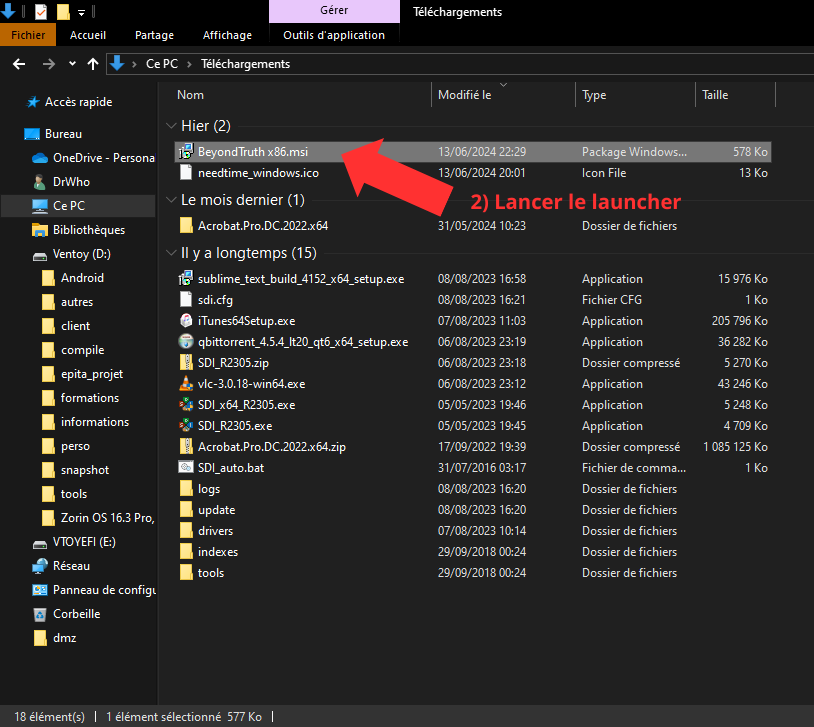
\includegraphics[width=1\linewidth]{start_launch.png}
	\legend{Téléchargement : \url{https://needtime.pages.dev/download}}
	
\end{figure}

\newpage

Vous devez poursuivre l'installation pour installer le jeu.

\vspace{0cm}
\begin{figure}[ht]
	\caption{Launcher}
	\centering
	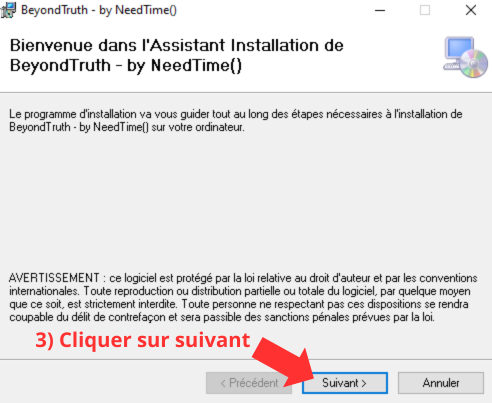
\includegraphics[width=1\linewidth]{launcher_1.png}
	\legend{Première fenêtre du launcher}
	
\end{figure}

\newpage

Vous pouvez configurer l'installation puis poursuivre avec les paramètres pour installer le jeu.

\vspace{0cm}
\begin{figure}[ht]
	\caption{Launcher}
	\centering
	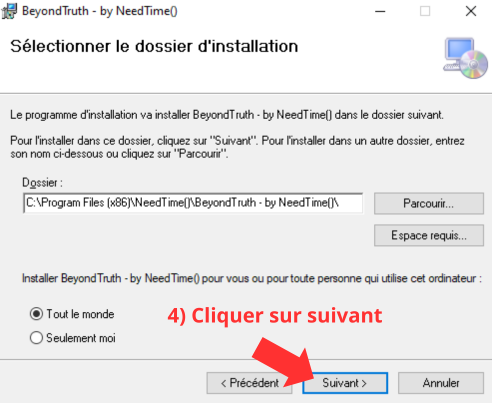
\includegraphics[width=1\linewidth]{launcher_2.png}
	\legend{Deuxième fenêtre du launcher}
	
\end{figure}

\newpage

Poursuivre l'installation du jeu pour pouvoir l'installer.

\vspace{0cm}
\begin{figure}[ht]
	\caption{Launcher}
	\centering
	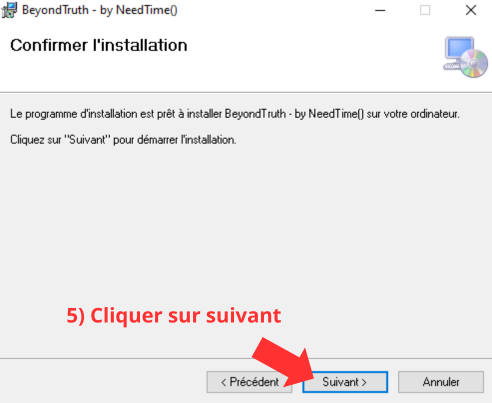
\includegraphics[width=1\linewidth]{launcher_3.png}
	\legend{Troisième fenêtre du launcher}
	
\end{figure}

\newpage

Il vous est enfin possible de lancer le jeu depuis le bureau ou le menu des applications Windows, l'installation du jeu est terminée.

\vspace{0cm}
\begin{figure}[ht]
	\caption{Launcher}
	\centering
	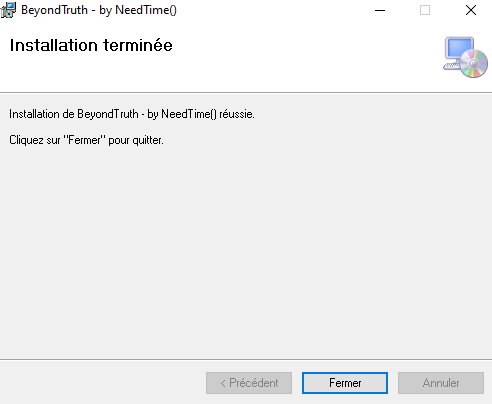
\includegraphics[width=1\linewidth]{installation_fin.png}
	\legend{Dernière fenêtre du launcher}
	
\end{figure}

\newpage

\section{Configuration minimale requise}

\begin{itemize}
    \item - Espace de stockage : 1 GB
    \item - RAM : 4 GB
    \item - CPU : Intel Core 2 Duo E8400
    \item - GPU : NVIDIA GeForce 6200
\end{itemize}

\section{Quels fichiers sont installés par le launcher ?}

Le launcher installe le jeu dans "C:/Program Files (x86)/NeedTime()/" et crée un raccourci dans "C:/ProgramData/Microsoft/Windows/Start Menu/Programs/BeyondTruth" et dans "C:/Users/Public/Desktop/BeyondTruth".

Les fichiers installés comprennent le logo au format .ico, l'exécutable du jeu au format .exe et les assets, le tout situé dans "C:/Program Files (x86)/NeedTime()/".

\newpage

\part{Comment désinstaller le jeu ?}

\section{Désinstallation par le launcher}

Pour désinstaller le jeu via le launcher, vous pouvez lancer le launcher d'installation et une procédure de désinstallation vous sera proposée.

\begin{figure}[ht]
    \caption{Launcher}
    \centering
    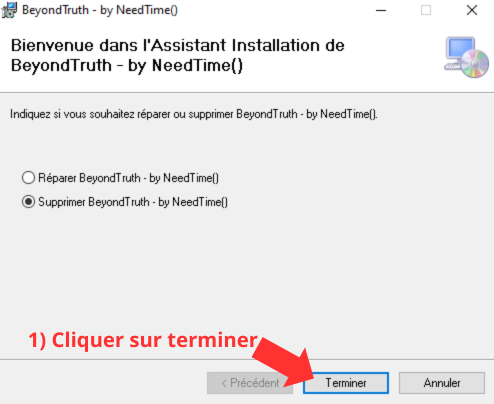
\includegraphics[width=1\linewidth]{uninstall_1.png}
    \legend{Première fenêtre du launcher}
    	
\end{figure}

\newpage

Patientez lors de la désinstallation.

\begin{figure}[ht]
    \caption{Launcher}
    \centering
    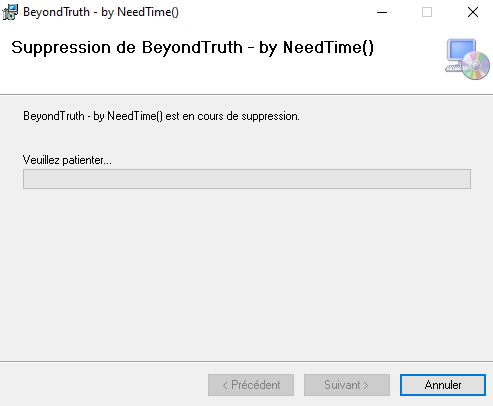
\includegraphics[width=1\linewidth]{supression.png}
    \legend{Deuxième fenêtre du launcher}
    	
\end{figure}

\newpage

Vous avez maintenant désinstallé le jeu, vous pouvez le réinstaller avec ce même launcher.

\begin{figure}[ht]
    \caption{Launcher}
    \centering
    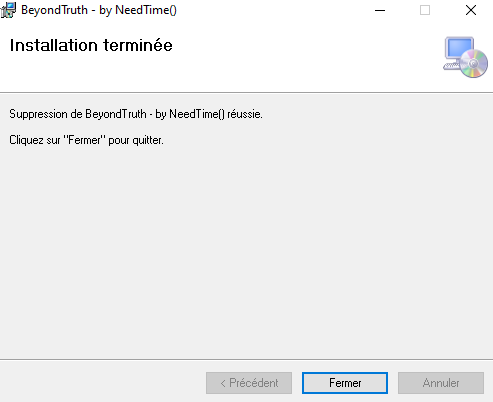
\includegraphics[width=1\linewidth]{supression_fin.png}
    \legend{Dernière fenêtre du launcher}
    	
\end{figure}

\section{Désinstallation via le menu windows}

Pour désinstaller le jeu via le menu windows, il faut vous rendre dans "Applications et fonctionnalités" rechercher le programme puis le désinstaller.

\vspace{0cm}
\begin{figure}[ht]
	\caption{Launcher}
	\centering
	\includegraphics[width=1\linewidth]{desinstallation_menu.png}
	\legend{Désinstallation via le menu windows}
	
\end{figure}

\newpage

\section{Désinstallation manuelle}

\begin{itemize}
    \item Supprimer le dossier situé dans "C:/Program Files (x86)/NeedTime()/"
    \vspace{0cm}
    \begin{figure}[ht]
    	\caption{Launcher}
    	\centering
    	\includegraphics[width=1\linewidth]{manuel_1.png}
    	\legend{Dossier du programme}
    	
    \end{figure}
    \newpage
    \item Supprimer le raccourci dans "C:/ProgramData/Microsoft/Windows/Start Menu/Programs/BeyondTruth"
    \vspace{0cm}
    \begin{figure}[ht]
    	\caption{Launcher}
    	\centering
    	\includegraphics[width=1\linewidth]{manuel_2.png}
    	\legend{Raccourci du programme}
    	
    \end{figure}
    \newpage
    \item Supprimer le raccourci dans "C:/Users/Public/Desktop/BeyondTruth"
    \vspace{0cm}
    \begin{figure}[ht]
    	\caption{Launcher}
    	\centering
    	\includegraphics[width=1\linewidth]{manuel_3.png}
    	\legend{Raccourci du programme}
    	
    \end{figure}
\end{itemize}

\newpage

\part{Comment utiliser le site ?}

\section{Visualiser le site en production}

Pour visualiser le site en production il suffit de vous rendre depuis un navigateur sur https://needtime.pages.dev/ :

\vspace{0cm}
\begin{figure}[ht]
	\caption{Aperçu du site}
	\centering
	\includegraphics[width=1\linewidth]{paper1.png}
	\legend{Site web: \url{https://needtime.pages.dev/}}
	
\end{figure}

\newpage

\section{Démarrer le site sur un serveur local}

Pour visualiser le site web sur un serveur de développement en local, vous pouvez utiliser le serveur de développement Servez disponible sur github (Linux, Windows, MacOS) :
\vspace{0cm}
\begin{figure}[ht]
	\caption{Servez}
	\centering
	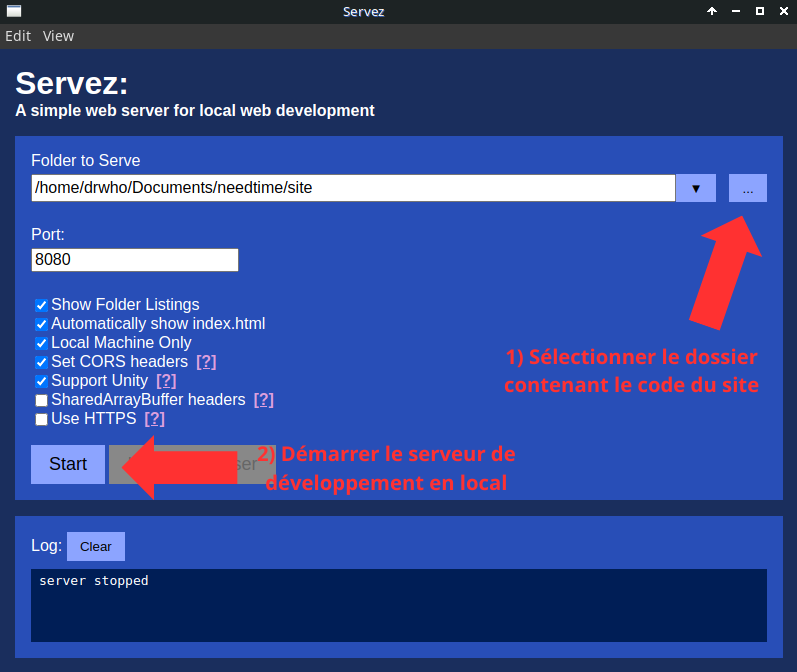
\includegraphics[width=1\linewidth]{dev_1.png}
	\legend{Téléchargement : \url{https://github.com/greggman/servez}}
	
\end{figure}

\newpage

Une fois la configuration effectuée il vous faut démarrer le serveur de développement web puis ouvrir un navigateur sur http://127.0.0.1:8080.

\vspace{0cm}
\begin{figure}[ht]
	\caption{Servez}
	\centering
	\includegraphics[width=1\linewidth]{dev_2.png}
	\legend{Téléchargement : \url{https://github.com/greggman/servez}}
	
\end{figure}

\newpage

\section{Indexation du site sur Google}

Nous avons optimisé les mots-clefs utilisés, la rapidité de chargement site ainsi que son contenu pour apparaître dans les premiers résultats de la recherche Google par référencement naturel.

\vspace{0cm}
\begin{figure}[ht]
	\caption{Indexation du site}
	\centering
	\includegraphics[width=1\linewidth]{indexation_site.png}
	\legend{Source: \url{https://google.com/}}
	
\end{figure}

\end{document}